\documentclass[10pt, a4paper, oneside, twocolumn]{report}

% encoding and language
\usepackage[utf8]{inputenc}
\usepackage[T1]{fontenc}
\usepackage[english]{babel}
\usepackage[babel]{csquotes}
\usepackage{subcaption}

% math packages
\usepackage{amsmath}
\usepackage{amsthm}
\usepackage{mathrsfs}
\usepackage{amssymb}

% graphics support
\usepackage{graphicx}
\usepackage{epsfig}
\usepackage{float}
\usepackage{color}

% nice tables
\usepackage{booktabs}

% hyperrefs
\usepackage{hyperref}

% metadata
\title{Bioinformatics Practicum\\\textbf{Project 5 - Phase Diagram of a Noble Gas}}
\author{Sebastian Hewett - Stephan Weißbach - Max Riedl - Laksan Nathan}
\date{\today}

\begin{document}
\maketitle

\chapter{Introduction to Molecular Dynamics Simulations}

Molecular dynamics (MD) is a computer simulation method for studying atoms and molecules in motion ~\cite{Gonzalez}. Following the laws of classical mechanics, i.e. numerically solving Newton's 2nd law (\ref{eq:2nd law}), MD simulations allow insights into trajectories for each atom \(i\) in a system constituted by \(N\) atoms. Forces between the particles and their potential energies are calculated using force fields.
%  this commented blank line prevents start of a new paragraph
\begin{equation}\label{eq:2nd law}
F_i = m_i a_i.
\end{equation} %  this commented blank line prevents start of a new paragraph
Here, \(m_i\) is the atom mass, \(a_i = \frac{d^{2}r_i}{d^{2}t}\) its acceleration, and \(F_i\) the force acting upon it, due to the interactions with other atoms.

Since molecular systems typically consist of a large number of particles, it is impossible to analytically determine the properties of such complex systems; MD simulation avoids this problem by using numerical methods. However, long MD simulations are mathematically ill-conditioned and produce cumulative errors in numerical integration. Proper selection of algorithms and parameters can mitigate this problem, but not completely eliminate it.

Analytical solutions are possible but time-consuming. Mostly, the error of approximation obtained with numerical solutions is acceptable. These numerical approaches enable solutions with a great number of very basic operations.

\section{Experiments}

It is necessary to understand the dynamics of a noble gas in order to understand its function. We first present our methodology and thought process on the set-up of such a MD simulation of argon atoms.

The system on which we conducted our simulations consisted of a simple single-atom particle enviroment, consisting of 100 (later of 216 atoms). Because of its inert state and single-atom nature, it does not create diatom structures as a gas or fluid (see: tutorial). It proves as a reliable candidate for the simulations where we only wanted to observe the dynamics of phase transition, without any interference through molecule formation or dipolar interactions. The experiment consited of three parts:
The transition from the gas state to the liquid state, then back to the gas state, and finally from the liquid to the solid state. The goal behind this was to observe the shift of potential energy thorughout the different transitions and its correlation with the temperature within the system. We also calculated the radial distribution of the argon atoms throughout the various states and the diffusion constant.

\section{Methods}

As our system particle we used argon with 100 atoms for the transition from gas to liquid and back to gas, and 216 atoms for the transition from liquid to solid. Since the simulation was run on a single-atom system, the force-field, where the only relevant terms were the Pauli-Repulsion and London-dispersion, could be kept very simple. The Pauli-Repulsion describes the force that prevents atoms from overlapping[1], while the London-dispersion describes the effects of induced dipol-dipol interaction[2]. The simulations were done with Gromacs. To simulate the various transitions we adjusted the temperatures accordingly. To validate
the outcome of the phase transition we visualized the simulation with PyMol, where the observations confirmed our assumptions.
We then extracted the potential and temperature curves with the gromacs "energy" command. For the diffusion constant we used "gmsd", while the radial distribution was calculated using "g". The plots were created with "xmgrace".

\chapter{Results}

The calculated diffusion constant is 2.5681 (+/- 0.1929) 10-5 \(cm^2/s\). Including the margin of error this result is as excepted. 

The diffusion coefficient the quantity of a substance that in diffusing from one region to another passes through each unit of cross section per unit of time when the volume-concentration gradient is unity—called also diffusivity.       

\begin{figure}
	\centering
		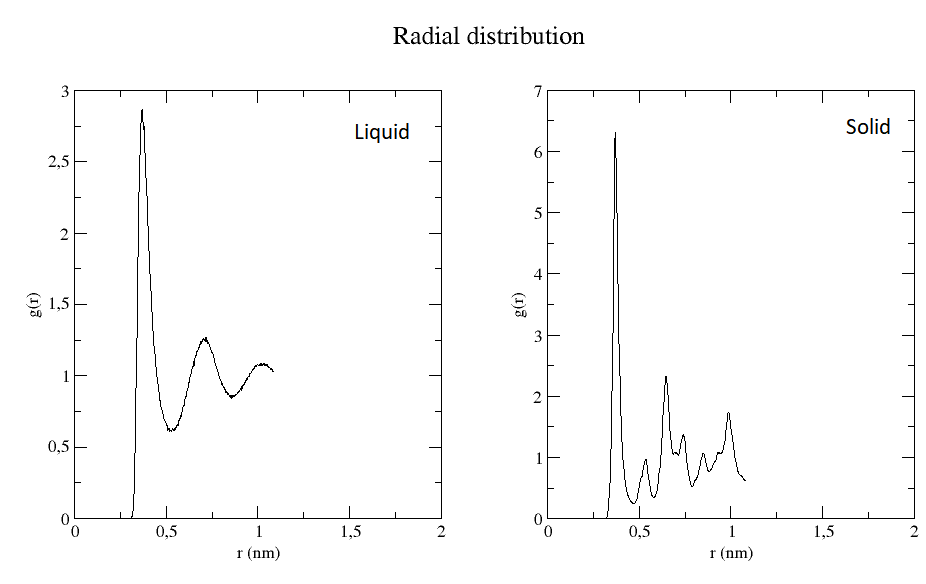
\includegraphics[width=\linewidth]{plots/rdf.png}
		\label{fig:1a}
\caption{Figure rdf from solid argon; correlation function against distance.}
\end{figure}

At both rdf before 0.3 there is zero correlation. The first peak is at r=0.37nm and g(r)=2.85 for liquid argon und g(r)=6.30 for solid argon, these are the highest peaks for each plot. In the liquid plot the next peak at 0.71nm. In the rdf plot for solid argon there is a small peak at r=0.54 with g(r) = 0.97 and a higher peak with g(r)=2.23 at r=0.65.

g(r) corrolation function, relation from bulk density(=average density) to local density(density from one molecule to an other) discribes the variation in density as a function of distance, so higher g(r) means more molecules at r.

Nearing r<3 the rdf is 0 as well for both states. This can be explained by the Lennard-Jones-Potential, because of the repulsion no two molecules are at close distance. The most molecules are at r=0.37, corresponding to the minimun in the LJP and experimental findings ~\cite{Argon, RDF}.
In solid state the peaks are higher and well defined, because the atoms are densly packed. The second (high > 0) peak appears at r=0.65 wich is roughly twice the distance from the center. This shows the constant structure of the solid phase. The broadening of the shape is because of vibrating of the molecules.In comparison the rdf of liquid argon shows the first peak ate the same r, but g(r) is half the size, which means less atoms at this given distance. The second peak is not at twice the distance as the first. Liquids are moore loosely packed so the intervals aren't as exact as in solids.

\section{Cooling}

In the first run, we cooled gaseous argon to a liquid state. We started with a fixed molecule count 100, a fixed volume and a starting tempreature of 100 degree Kelvin. Over 5000 picoseconds we decreased the tempreature with a thermostat to 25 Kelvin. As we slowly decrease the temperature the system is losing kinetic energy. Due to the decrease of total energy in the system, the potential energy also decreases.
The potential energy of atoms at higher temperatures is stored by electrons in excited states, additionally at higher temperatures more atoms are in excited rotationally states. ~\cite{chemguide}
The virial theorem specifies, that the potential energy and the kinetic energy in a system are depend on each other. ~\cite{cosmos-indirekt}
The phase transition was between 3000 and 4500 picoseconds and is characterized by a strong drop in potential energy. 

\begin{figure}
	\begin{subfigure}[HB!]{0.5\textwidth}
		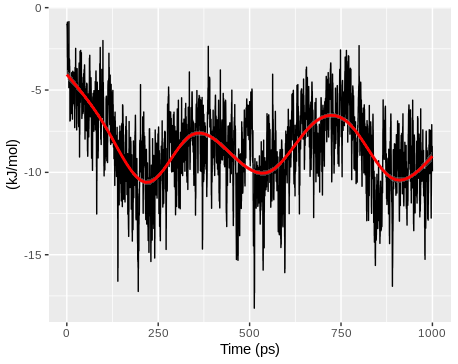
\includegraphics[width=0.85\textwidth]{plots/potential_energy.png}
		\subcaption{x-axis: time in picoseconds; y-axis: po-
			tential energy in kilojoule per mol}
	\end{subfigure}
	\begin{subfigure}[HB!]{0.5\textwidth}
		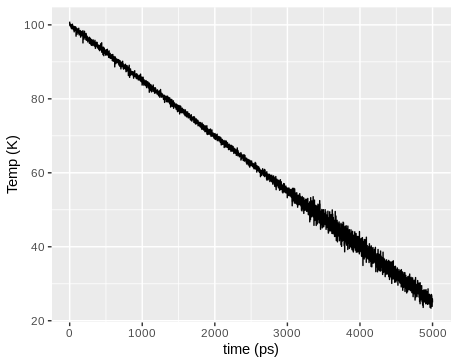
\includegraphics[width=0.85\textwidth]{plots/temp_plot.png}
		\subcaption{x-axis: time in picoseconds; y-axis: tem-
			perature in Kelvin}
	\end{subfigure}
	\caption{Simulation of cooling Argon from gaseous to liquid state.}
\end{figure}

\section{Freezing}

Next, we cooled liquid argon to a solid state. We started with an increased molecule count of 216 Argon atoms, a fixed volume (not changed) and a starting tempreature of 100 degree Kelvin. Due to the increased molecule count and not changed volumen the pressure was much higher. Again we can obsorve a drop in potential energy during the phase transition to solid, but this time it faster (300 and 500 picoseconds).

\begin{figure}
	\begin{subfigure}[HB!]{0.5\textwidth}
	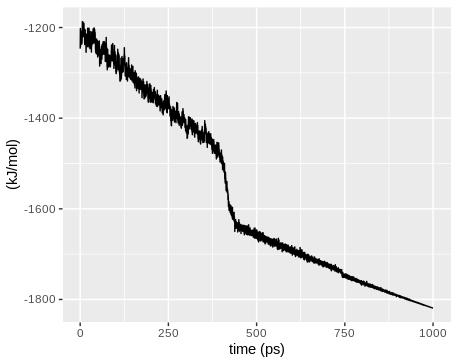
\includegraphics[width=0.85\textwidth]{plots//freezing/freezing_pot_en.png}
    \caption{x-axis: time in picoseconds; y-axis: po-
    	tential energy in kilojoule per mol.}
\end{subfigure}
	\begin{subfigure}[HB!]{0.5\textwidth}
	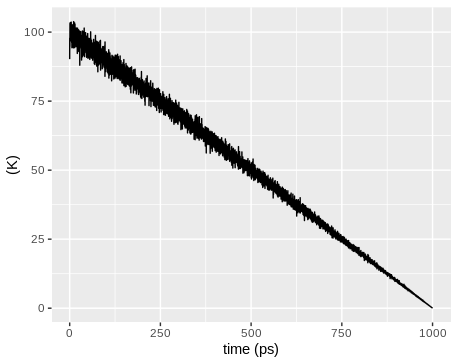
\includegraphics[width=0.85\textwidth]{plots//freezing/freezing_temp.png}
    \caption{x-axis: time in picoseconds; y-axis: tem-
    	perature in Kelvin.}
\end{subfigure}
\caption{Simulation of cooling Argon from liquid to solid}
\end{figure}

\section{Heat-Up}

At last we simulated the heat up of liquid Argon to gaseous state. We ran the simulation with 100 Argon atoms, a fixed volume and a starting tempreature of 50 degree Kelvin. Over 5000 picoseconds we increased the tempreature with a thermostat to 125 degree Kelvin.
The potential energy plot has a higher variance, which might be related to the use of a thermostat. This sets the temperature (= the kinetic energy) of atoms to a desired value. If an atom is accelerated by potential energy consumption, it can be slowed down again by the thermostat. This would lead to a loss of energy. Another effect could be explained by the non-simultaneous phase transition.

\begin{figure}
	\begin{subfigure}[HB!]{0.5\textwidth}
		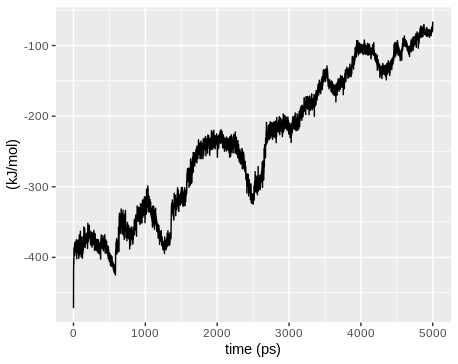
\includegraphics[width=0.85\textwidth]{plots/Heatup/pot_energy_heatup.png}
		\caption{x-axis: time in picoseconds; y-axis: potential energy in kilojoule per mol}
	\end{subfigure}
	\begin{subfigure}[HB!]{0.5\textwidth}
		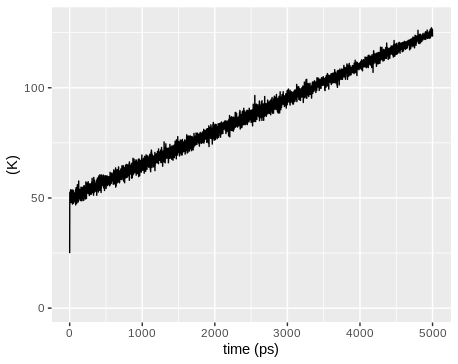
\includegraphics[width=0.85\textwidth]{plots/Heatup/temp_heatup.png}
		\caption{x-axis: time in picoseconds; y-axis: temperature in Kelvin}
	\end{subfigure}
	\caption{Simulation of heating Argon from liquid to gaseous}
\end{figure}

\begin{thebibliography}{100}
\bibitem{Gonzalez} M.A.González: Force fields and molecular dynamics simulations. \textit{JDN}, Volume 12, 2011. 169 - 200. 2011.
\bibitem{Quant} P. A. M. Dirac: On the Theory of Quantum Mechanics, \textit{Proceedings of the Royal Society of London}, Series A 112, pp. 661—677. 1926.
\bibitem{Molekular} London, F.: Zur Theorie und Systematik der Molekularkräfte. 1930. 
\bibitem{chemguide}  \hyperlink{http://www.chemguide.co.uk/analysis/uvvisible/theory.html}{UV-visible absorption spectra [chemguide.co.uk]} (Zugegriffen am 21.03.2019 um 15:20 Uhr).
\bibitem{cosmos-indirekt} \hyperlink{https://physik.cosmos-indirekt.de/Physik-Schule/Virialsatz}{Virialsatz [physik.comsoms-indirekt.de]} (Zugegriffen am 21.03.2019 um 15:30 Uhr)
\bibitem{Argon} \hyperlink{http://www.sklogwiki.org/SklogWiki/index.php/Argon}{Argon}(Zugegriffen am 21.03.2019 um 15:23 Uhr)
\bibitem{RDF} \hyperlink{https://www.ncbi.nlm.nih.gov/pmc/articles/PMC349093/?page=4}{RDF}(Zugegriffen am 21.03.2019 um 9:09 Uhr)
\end{thebibliography}

\end{document}


